\documentclass[twoside]{book}

% Packages required by doxygen
\usepackage{fixltx2e}
\usepackage{calc}
\usepackage{doxygen}
\usepackage[export]{adjustbox} % also loads graphicx
\usepackage{graphicx}
\usepackage[utf8]{inputenc}
\usepackage{makeidx}
\usepackage{multicol}
\usepackage{multirow}
\PassOptionsToPackage{warn}{textcomp}
\usepackage{textcomp}
\usepackage[nointegrals]{wasysym}
\usepackage[table]{xcolor}

% Font selection
\usepackage[T1]{fontenc}
\usepackage[scaled=.90]{helvet}
\usepackage{courier}
\usepackage{amssymb}
\usepackage{sectsty}
\renewcommand{\familydefault}{\sfdefault}
\allsectionsfont{%
  \fontseries{bc}\selectfont%
  \color{darkgray}%
}
\renewcommand{\DoxyLabelFont}{%
  \fontseries{bc}\selectfont%
  \color{darkgray}%
}
\newcommand{\+}{\discretionary{\mbox{\scriptsize$\hookleftarrow$}}{}{}}

% Page & text layout
\usepackage{geometry}
\geometry{%
  a4paper,%
  top=2.5cm,%
  bottom=2.5cm,%
  left=2.5cm,%
  right=2.5cm%
}
\tolerance=750
\hfuzz=15pt
\hbadness=750
\setlength{\emergencystretch}{15pt}
\setlength{\parindent}{0cm}
\setlength{\parskip}{3ex plus 2ex minus 2ex}
\makeatletter
\renewcommand{\paragraph}{%
  \@startsection{paragraph}{4}{0ex}{-1.0ex}{1.0ex}{%
    \normalfont\normalsize\bfseries\SS@parafont%
  }%
}
\renewcommand{\subparagraph}{%
  \@startsection{subparagraph}{5}{0ex}{-1.0ex}{1.0ex}{%
    \normalfont\normalsize\bfseries\SS@subparafont%
  }%
}
\makeatother

% Headers & footers
\usepackage{fancyhdr}
\pagestyle{fancyplain}
\fancyhead[LE]{\fancyplain{}{\bfseries\thepage}}
\fancyhead[CE]{\fancyplain{}{}}
\fancyhead[RE]{\fancyplain{}{\bfseries\leftmark}}
\fancyhead[LO]{\fancyplain{}{\bfseries\rightmark}}
\fancyhead[CO]{\fancyplain{}{}}
\fancyhead[RO]{\fancyplain{}{\bfseries\thepage}}
\fancyfoot[LE]{\fancyplain{}{}}
\fancyfoot[CE]{\fancyplain{}{}}
\fancyfoot[RE]{\fancyplain{}{\bfseries\scriptsize Generated by Doxygen }}
\fancyfoot[LO]{\fancyplain{}{\bfseries\scriptsize Generated by Doxygen }}
\fancyfoot[CO]{\fancyplain{}{}}
\fancyfoot[RO]{\fancyplain{}{}}
\renewcommand{\footrulewidth}{0.4pt}
\renewcommand{\chaptermark}[1]{%
  \markboth{#1}{}%
}
\renewcommand{\sectionmark}[1]{%
  \markright{\thesection\ #1}%
}

% Indices & bibliography
\usepackage{natbib}
\usepackage[titles]{tocloft}
\setcounter{tocdepth}{3}
\setcounter{secnumdepth}{5}
\makeindex

% Hyperlinks (required, but should be loaded last)
\usepackage{ifpdf}
\ifpdf
  \usepackage[pdftex,pagebackref=true]{hyperref}
\else
  \usepackage[ps2pdf,pagebackref=true]{hyperref}
\fi
\hypersetup{%
  colorlinks=true,%
  linkcolor=blue,%
  citecolor=blue,%
  unicode%
}

% Custom commands
\newcommand{\clearemptydoublepage}{%
  \newpage{\pagestyle{empty}\cleardoublepage}%
}

\usepackage{caption}
\captionsetup{labelsep=space,justification=centering,font={bf},singlelinecheck=off,skip=4pt,position=top}

%===== C O N T E N T S =====

\begin{document}

% Titlepage & ToC
\hypersetup{pageanchor=false,
             bookmarksnumbered=true,
             pdfencoding=unicode
            }
\pagenumbering{alph}
\begin{titlepage}
\vspace*{7cm}
\begin{center}%
{\Large My Project }\\
\vspace*{1cm}
{\large Generated by Doxygen 1.8.13}\\
\end{center}
\end{titlepage}
\clearemptydoublepage
\pagenumbering{roman}
\tableofcontents
\clearemptydoublepage
\pagenumbering{arabic}
\hypersetup{pageanchor=true}

%--- Begin generated contents ---
\chapter{Class Index}
\section{Class List}
Here are the classes, structs, unions and interfaces with brief descriptions\+:\begin{DoxyCompactList}
\item\contentsline{section}{\hyperlink{struct__Btree}{\+\_\+\+Btree} }{\pageref{struct__Btree}}{}
\item\contentsline{section}{\hyperlink{struct__CumCol3}{\+\_\+\+Cum\+Col3} }{\pageref{struct__CumCol3}}{}
\item\contentsline{section}{\hyperlink{struct__CumCol4}{\+\_\+\+Cum\+Col4} }{\pageref{struct__CumCol4}}{}
\item\contentsline{section}{\hyperlink{struct__Data}{\+\_\+\+Data} }{\pageref{struct__Data}}{}
\end{DoxyCompactList}

\chapter{Class Documentation}
\hypertarget{struct__Btree}{}\section{\+\_\+\+Btree Struct Reference}
\label{struct__Btree}\index{\+\_\+\+Btree@{\+\_\+\+Btree}}


Collaboration diagram for \+\_\+\+Btree\+:
\nopagebreak
\begin{figure}[H]
\begin{center}
\leavevmode
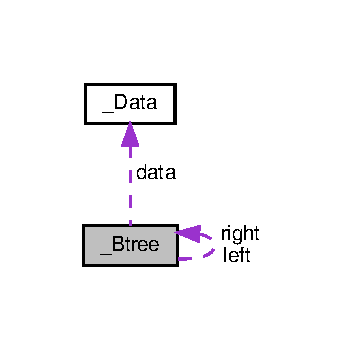
\includegraphics[width=165pt]{struct__Btree__coll__graph}
\end{center}
\end{figure}
\subsection*{Public Attributes}
\begin{DoxyCompactItemize}
\item 
\mbox{\Hypertarget{struct__Btree_a8f210f6335be3cf206adbcfd390dd4bc}\label{struct__Btree_a8f210f6335be3cf206adbcfd390dd4bc}} 
\hyperlink{struct__Data}{Data} {\bfseries data}
\item 
\mbox{\Hypertarget{struct__Btree_a25f05500ebe2cf740236e1aa18d9e085}\label{struct__Btree_a25f05500ebe2cf740236e1aa18d9e085}} 
struct \hyperlink{struct__Btree}{\+\_\+\+Btree} $\ast$ {\bfseries left}
\item 
\mbox{\Hypertarget{struct__Btree_a4dd47df91cb75b5884d36cb95b7ec3eb}\label{struct__Btree_a4dd47df91cb75b5884d36cb95b7ec3eb}} 
struct \hyperlink{struct__Btree}{\+\_\+\+Btree} $\ast$ {\bfseries right}
\end{DoxyCompactItemize}


The documentation for this struct was generated from the following file\+:\begin{DoxyCompactItemize}
\item 
library.\+h\end{DoxyCompactItemize}

\hypertarget{struct__CumCol3}{}\section{\+\_\+\+Cum\+Col3 Struct Reference}
\label{struct__CumCol3}\index{\+\_\+\+Cum\+Col3@{\+\_\+\+Cum\+Col3}}


Collaboration diagram for \+\_\+\+Cum\+Col3\+:
\nopagebreak
\begin{figure}[H]
\begin{center}
\leavevmode
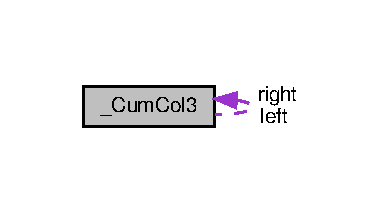
\includegraphics[width=183pt]{struct__CumCol3__coll__graph}
\end{center}
\end{figure}
\subsection*{Public Attributes}
\begin{DoxyCompactItemize}
\item 
\mbox{\Hypertarget{struct__CumCol3_a95a7df966f21674b1f0cb8db80392f07}\label{struct__CumCol3_a95a7df966f21674b1f0cb8db80392f07}} 
char $\ast$ {\bfseries analyze}
\item 
\mbox{\Hypertarget{struct__CumCol3_ac9a1ae1b2a650947393ade7c945dec08}\label{struct__CumCol3_ac9a1ae1b2a650947393ade7c945dec08}} 
float {\bfseries prob}
\item 
\mbox{\Hypertarget{struct__CumCol3_afc3e3ea07d91ef3b3f1711d33db466cb}\label{struct__CumCol3_afc3e3ea07d91ef3b3f1711d33db466cb}} 
int {\bfseries count}
\item 
\mbox{\Hypertarget{struct__CumCol3_af85f116f5acf778c909c173947408573}\label{struct__CumCol3_af85f116f5acf778c909c173947408573}} 
struct \hyperlink{struct__CumCol3}{\+\_\+\+Cum\+Col3} $\ast$ {\bfseries left}
\item 
\mbox{\Hypertarget{struct__CumCol3_afe4e71d5bd088eaac03ce49e1e054b4d}\label{struct__CumCol3_afe4e71d5bd088eaac03ce49e1e054b4d}} 
struct \hyperlink{struct__CumCol3}{\+\_\+\+Cum\+Col3} $\ast$ {\bfseries right}
\end{DoxyCompactItemize}


The documentation for this struct was generated from the following file\+:\begin{DoxyCompactItemize}
\item 
library.\+h\end{DoxyCompactItemize}

\hypertarget{struct__CumCol4}{}\section{\+\_\+\+Cum\+Col4 Struct Reference}
\label{struct__CumCol4}\index{\+\_\+\+Cum\+Col4@{\+\_\+\+Cum\+Col4}}


Collaboration diagram for \+\_\+\+Cum\+Col4\+:
\nopagebreak
\begin{figure}[H]
\begin{center}
\leavevmode
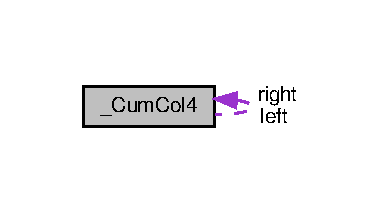
\includegraphics[width=183pt]{struct__CumCol4__coll__graph}
\end{center}
\end{figure}
\subsection*{Public Attributes}
\begin{DoxyCompactItemize}
\item 
\mbox{\Hypertarget{struct__CumCol4_a0836e5d720571263a910ade8b0b61b22}\label{struct__CumCol4_a0836e5d720571263a910ade8b0b61b22}} 
char $\ast$ {\bfseries analyze}
\item 
\mbox{\Hypertarget{struct__CumCol4_a9ad9ad1d2806348025be19e97bc189d3}\label{struct__CumCol4_a9ad9ad1d2806348025be19e97bc189d3}} 
float {\bfseries prob}
\item 
\mbox{\Hypertarget{struct__CumCol4_a739585d1fabbaaf1104d096de42c074d}\label{struct__CumCol4_a739585d1fabbaaf1104d096de42c074d}} 
int {\bfseries count}
\item 
\mbox{\Hypertarget{struct__CumCol4_af7b17f86fb4f71c18465e3fdbf8c82de}\label{struct__CumCol4_af7b17f86fb4f71c18465e3fdbf8c82de}} 
float {\bfseries media}
\item 
\mbox{\Hypertarget{struct__CumCol4_a2a45de85bb6919d763919435b0928106}\label{struct__CumCol4_a2a45de85bb6919d763919435b0928106}} 
float {\bfseries Str\+Dev}
\item 
\mbox{\Hypertarget{struct__CumCol4_a41814f047c2f8082bd835a0c92ca6964}\label{struct__CumCol4_a41814f047c2f8082bd835a0c92ca6964}} 
float {\bfseries total\+Str\+Dev}
\item 
\mbox{\Hypertarget{struct__CumCol4_ac689ab32b082fde43c793ea80325683b}\label{struct__CumCol4_ac689ab32b082fde43c793ea80325683b}} 
struct \hyperlink{struct__CumCol4}{\+\_\+\+Cum\+Col4} $\ast$ {\bfseries left}
\item 
\mbox{\Hypertarget{struct__CumCol4_ae534286d0dbaf7676165270584071f38}\label{struct__CumCol4_ae534286d0dbaf7676165270584071f38}} 
struct \hyperlink{struct__CumCol4}{\+\_\+\+Cum\+Col4} $\ast$ {\bfseries right}
\end{DoxyCompactItemize}


The documentation for this struct was generated from the following file\+:\begin{DoxyCompactItemize}
\item 
library.\+h\end{DoxyCompactItemize}

\hypertarget{struct__Data}{}\section{\+\_\+\+Data Struct Reference}
\label{struct__Data}\index{\+\_\+\+Data@{\+\_\+\+Data}}
\subsection*{Public Attributes}
\begin{DoxyCompactItemize}
\item 
\mbox{\Hypertarget{struct__Data_a9a1f93b633bb116da8a09169c2475651}\label{struct__Data_a9a1f93b633bb116da8a09169c2475651}} 
char $\ast$ {\bfseries word}
\item 
\mbox{\Hypertarget{struct__Data_ad03e2970d95fbd4128d0fda12cd94844}\label{struct__Data_ad03e2970d95fbd4128d0fda12cd94844}} 
char $\ast$ {\bfseries motto}
\item 
\mbox{\Hypertarget{struct__Data_a70d8e1db27f9c6bc12102527fd585e0a}\label{struct__Data_a70d8e1db27f9c6bc12102527fd585e0a}} 
char $\ast$ {\bfseries analyze}
\item 
\mbox{\Hypertarget{struct__Data_a0eb20cfcb1816e9eb4b41e45b981dcd9}\label{struct__Data_a0eb20cfcb1816e9eb4b41e45b981dcd9}} 
float {\bfseries prob}
\item 
\mbox{\Hypertarget{struct__Data_aad34f3ac5590099c8bce026e115c8e53}\label{struct__Data_aad34f3ac5590099c8bce026e115c8e53}} 
int {\bfseries total\+Occurrences}
\item 
\mbox{\Hypertarget{struct__Data_a94bd7619e92c5ce3369c2b94a9e3048f}\label{struct__Data_a94bd7619e92c5ce3369c2b94a9e3048f}} 
int {\bfseries lenght\+Word}
\end{DoxyCompactItemize}


The documentation for this struct was generated from the following file\+:\begin{DoxyCompactItemize}
\item 
library.\+h\end{DoxyCompactItemize}

%--- End generated contents ---

% Index
\backmatter
\newpage
\phantomsection
\clearemptydoublepage
\addcontentsline{toc}{chapter}{Index}
\printindex

\end{document}
